%\documentclass{article}
%\usepackage{graphicx,subfigure}
%\begin{document}

\begin{figure}[!h]
  \centering
  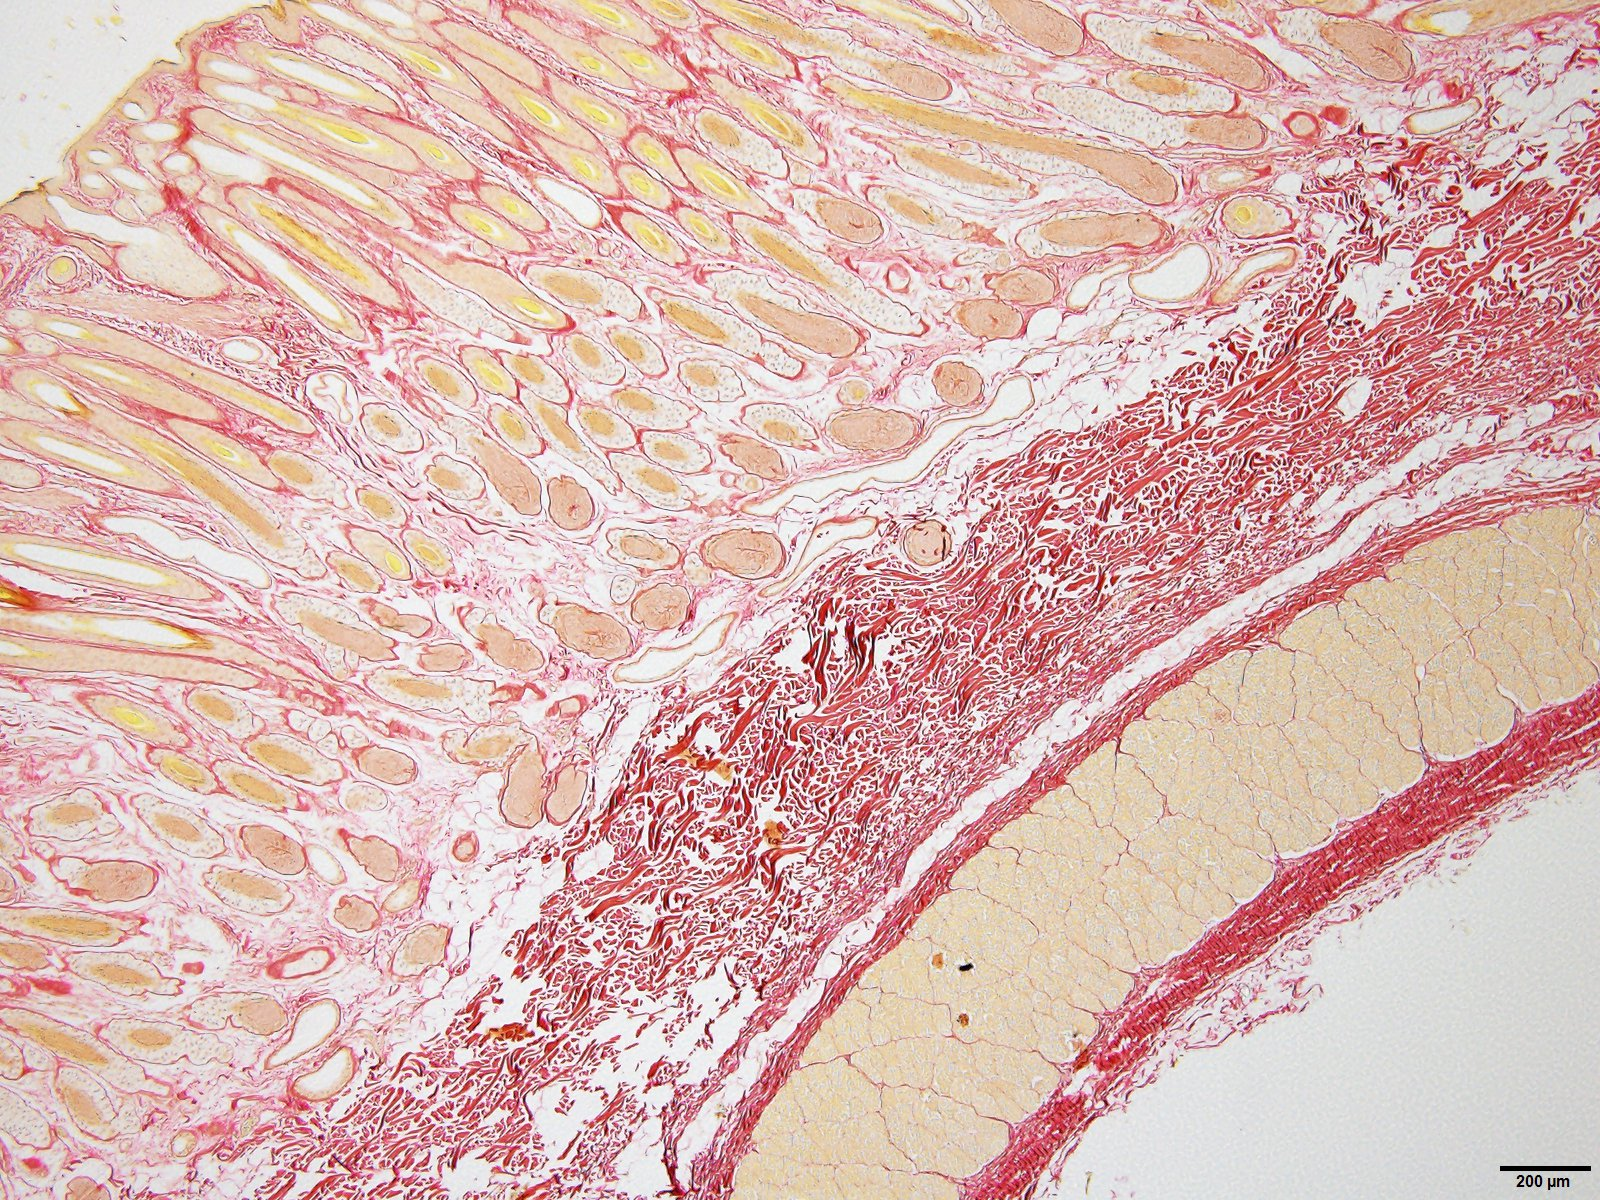
\includegraphics[width=1.0\textwidth]{3456_4layers_4x_PSR.jpg}
  \caption{Vertical section from a wrinkled sheep (3456) from Trial 2 Flock 1 stained with PSR and viewed with bright field microscope. This section is from an untrimmed biopsy specimen and shows all 4 layers (Epidermis, Papillary dermis, Reticular dermis and Muscle layer). Collagen (stained red) is present in Layers 2 and 3, and on the borders of Layer 4}
  \label{fig:trial2psr}
\end{figure}

%\end{document}

